\documentclass[12t,a4paper]{article}
\usepackage{listings}
\usepackage{graphicx}
\usepackage[utf8]{inputenc}
\usepackage{listings}
\usepackage{wrapfig}
\usepackage{url}
\usepackage{amsmath}
\usepackage{caption}
\usepackage{setspace}
\usepackage[left=2cm,right=2cm,top=2cm,bottom=2cm]{geometry}

\onehalfspacing

\title{Stage Android : Infos pratiques et support théorique}
\author{Encadrants : Pierre-Olivier Colard et Florian Demesmaeker}
\date{01/08/2016 - 05/08/2016}

%
%
% Auteurs : 
% Pierre-Olivier Colard
% Florian Demesmaeker
%
%

\begin{document}

\maketitle
\begin{center}
\begin{figure}[h!]

\includegraphics[width=1\linewidth]{android_logo.jpg}
\end{figure}
\end{center}

\vfill

\begin{minipage}{0.3\linewidth}

\includegraphics[scale=0.25]{tic_logo.jpg}
\end{minipage}
\hfill
\begin{minipage}{0.3\linewidth}

\includegraphics[scale=0.25]{epl-logo.jpg}
\end{minipage}
\hfill
\begin{minipage}{0.3\linewidth}

\includegraphics[scale=0.25]{ucl-logo.jpg}
\end{minipage}

\thispagestyle{empty}
\setcounter{page}{0}
\newpage

\tableofcontents
\clearpage

\section{Planning}

Bienvenue ! Voici le planning de cette semaine de stage.

\subsection{Lundi}
\textbf{Matin}~ Présentation générale, présentation d'Android et d'App Inventor 2. Projet Miaou. \\
\textbf{Après-midi}~ Théorie si-sinon et variables. Projet PlusOuMoins. Bonus : mot de passe.

\subsection{Mardi}
\textbf{Matin}~ Théorie Horloges. Projet décompte. Théorie procédure. Projet SayMyName. \\
\textbf{Après-midi}~ Plusieurs projets : calculatrice, touches de piano.

\subsection{Mercredi}
\textbf{Matin}~ Présentation des images lutins, des animations, des déplacements et des collisions. \\
\textbf{Après-midi}~ Projets : Space invaders ou casse-brique. Consignes pour le projet final.

\subsection{Jeudi}
\textbf{Matin}~ Conception de votre application \textbf{sur papier}. \\
\textbf{Après-midi}~ Implémentation de votre application !

\subsection{Vendredi}
\textbf{Matin}~ Finalisation de votre application et publication des plus évoluées. \\
\textbf{Après-midi}~ Derniers détails de votre application et présentation aux parents.

\vfill

\begin{figure}[h!]
\begin{center}

\includegraphics[scale=0.5]{schedule.png}
\end{center}
\end{figure}


\newpage

\section{Présentation de App Inventor 2}

App Inventor est un logiciel développé par le MIT pour simplifier la création d'applications Android. Son utilisation ne nécessite aucune base en programmation. Au lieu de lignes de code, on emboite des blocs pour programmer. Pour y accéder, entrez \url{http://ai2.appinventor.mit.edu} dans votre navigateur favori.

Pour créer un projet, il suffit d'appuyer sur le bouton \texttt{Commencer un nouveau projet...} dans la vue générale d'App Inventor~: 

\begin{figure}[h!]
\begin{center}
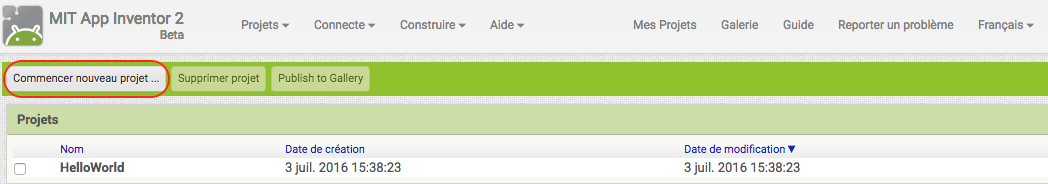
\includegraphics[scale=0.46]{newProject.png}
\end{center}
\end{figure}

Nous arrivons ensuite sur la vue \textbf{Designer}:
\begin{figure}[h!]
\begin{center}
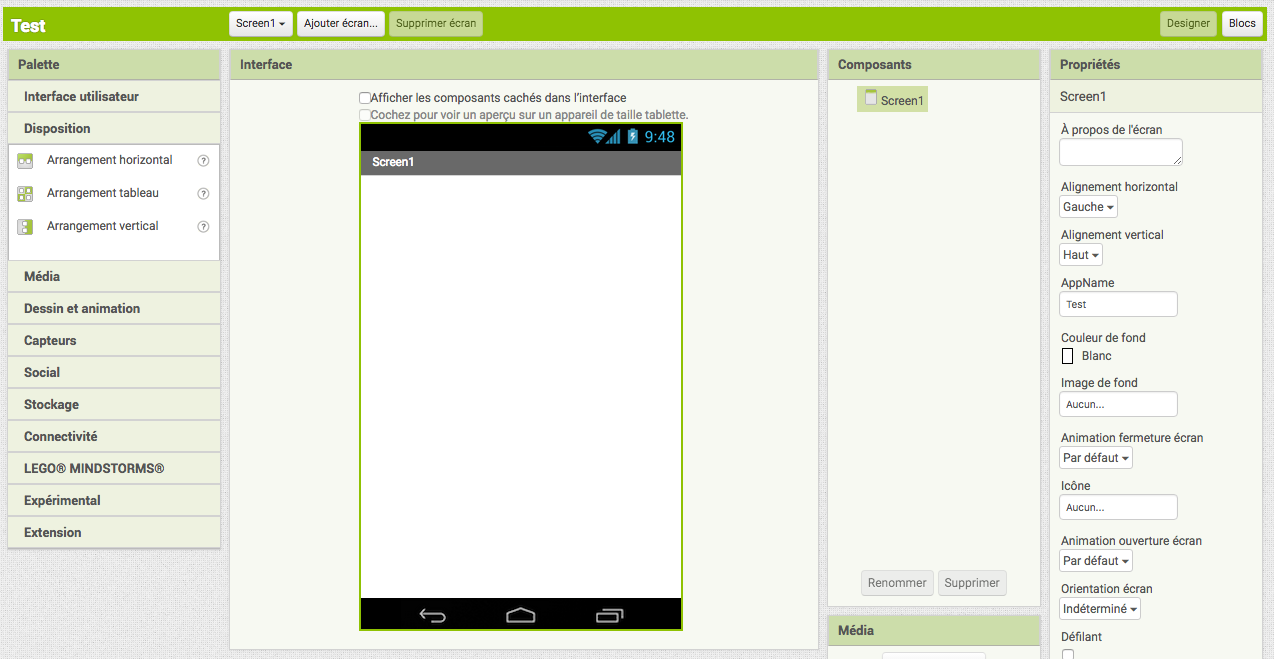
\includegraphics[scale=0.38]{VueDesigner2.png}
\end{center}
\end{figure}

C'est sur cet écran que l'on contruit l'\textit{interface} de notre application. Comment faire ? Nous pouvons chercher les éléments que l'on veut placer sur notre écran dans la Palette et les amener sur l'\textbf{Interface}. Par exemple, pour rajouter un bouton sur l'écran, on cherche \textbf{Bouton} dans le menu \textbf{Interface Utilisateur} de la \textbf{Palette}, on clique ensuite sur \textbf{Bouton} et sans lâcher le clic, on le déplace jusque dans l'\textbf{Interface}. \\

Nous pouvons placer toute une série d'éléments dans l'\textbf{Interface}, comme des boutons, des images et des listes, mais aussi des éléments invisibles qui nous serviront par la suite, comme un minuteur, un son, un objet de reconnaissance vocale,... On peut également organiser tous ces éléments en utilisant des \textbf{Arrangements horizontaux}, \textbf{Arrangements verticaux} ou des \textbf{Arrangements tableaux} disponibles dans le menu \textbf{Disposition} de la \textbf{Palette}.\\

Enfin, on observe aussi à droite de l'\textbf{Interface} la colonne \textbf{Composants} et la colonne \textbf{Propriétés}. Dans \textbf{Composants}, on retrouve un résumé de tous les objets placés dans l'\textbf{Interface}. C'est là qu'on peut changer le nom par lequel on désigne nos objets, par exemple changer \textit{Button1} en \textit{Bouton Start}. Dans \textbf{Propriétés}, on peut changer toutes les caractéristiques d'un objet placé dans l'\textbf{Interface}. Par exemple pour l'horloge, on peut déterminer si elle est activée par défaut (\textbf{ChronomètreActivé}), si elle s'exécute tout le temps (\textbf{TimerAlwaysFire}) et sa longueur (\textbf{IntervalleChronomètre}). Pour un \textbf{Bouton}, on peut déterminer le texte, la taille, la couleur, etc.\\

Pour  pouvoir programmer, on passe dans la vue des \textbf{Blocs} (juste au-dessus de \textbf{Propriétés} quand on est dans le \textbf{Designer})~:
\begin{figure}[h!]
\begin{center}
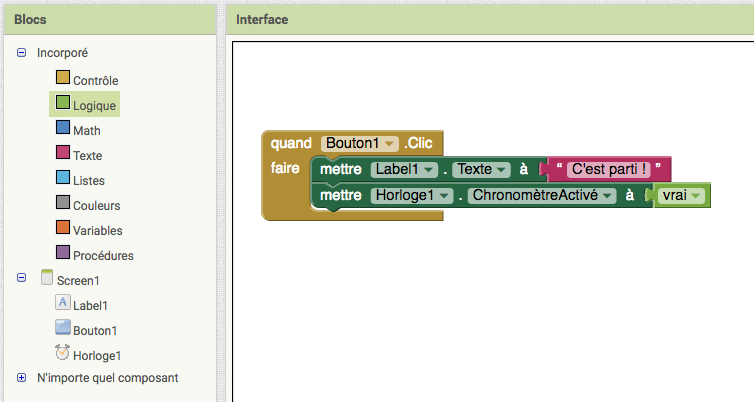
\includegraphics[scale=0.5]{Blocks.png}
\end{center}
\end{figure}

Dans cette seconde vue, on peut effectuer des actions sur les objets placés dans la vue \textbf{Designer}, ou dépendant de ces objets. Par exemple, en cliquant sur \textbf{Button1}, le bloc \texttt{Quand Button1.Clic faire} apparait, entre autres. Pour l'utiliser, il suffit de le déplacer dans l'\textbf{Interface}. Toute une série d'actions (toujours sous forme de blocs) est possible pour chaque objet.\\

Les actions plus générales sont accessibles depuis le menu \textbf{Incorporé} dans les \textbf{Blocs}. 
\begin{itemize}
\item Dans \textbf{Contrôle}, on retrouve les boucles, les structures conditionnelles et la gestion des écrans et de l'application en général. 
\item Dans \textbf{Logique}, on retrouve les opérations logiques (vrai, faux, et, ou,...)
\item Dans \textbf{Math}, on a toutes les opérations mathématiques disponibles.
\item Dans \textbf{Texte}, on a toute la gestion du texte, telle que concaténer des textes (assembler deux textes en un), vérifier la longueur d'un texte, écrire un texte, etc.
\item Dans \textbf{Listes}, on a toute la gestion des listes.
\item Dans \textbf{Couleurs}, on retrouve toutes les couleurs disponibles.
\item Dans \textbf{Variables}, on a les blocs nécessaires à l'utilisation de variables.
\item Dans \textbf{Procédures}, on a les blocs nécessaires à la création de fonctions (qu'on n'utilisera a priori pas cette semaine).
\end{itemize}



\newpage

\section{Support théorique et exemples pratiques}
\subsection{Les variables}
Les variables sont un des concepts de base de l'informatique. Il s'agit de cases mémoires possédant chacune un nom pour la désigner, ainsi qu'un contenu. Le nom d'une variable ne change jamais. Une fois que la variable est déclarée, un nom lui est donné une fois pour toutes. Le contenu de la variable peut quant à lui être régulièrement changé.\\

Dans App Inventor, les variables peuvent être utilisées grâce à des blocs. Les deux premières choses qu'on doit faire lorsque l'on utilise des variables sont~: les déclarer (leur donner un nom) et les initialiser (leur donner un contenu). Dans App Inventor, ces deux actions sont exécutées par un seul bloc:

\begin{figure}[h!]
\centering
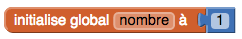
\includegraphics[scale=0.6]{Initialisation.png}
\end{figure}

Ici, on a créé une variable que l'on a appelé \textit{nombre} et qui contient la valeur $1$.\\

On peut utiliser le contenu d'une variable en prenant le bloc orange \textit{obtenir "le nom de la variable"}~:
\begin{figure}[h!]
\centering
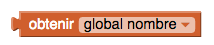
\includegraphics[scale=0.6]{get.png}
\end{figure}

On peut également modifier son contenu en prenant le bloc orange \textit{mettre "le nom de la variable" "le nouveau contenu"}~:
\begin{figure}[h!]
\centering
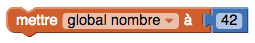
\includegraphics[scale=0.6]{set.png}
\end{figure}

Par exemple ici on augmente la valeur de \textit{nombre} de 1. Pouvez-vous expliquer comment on s'y prend~?

\begin{figure}[h!]
\centering
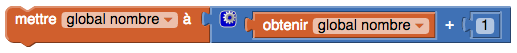
\includegraphics[scale=0.6]{set2.png}
\end{figure}



\subsection{Les structures conditionnelles}

Derrière ce nom qui peut sembler un peu barbare à première vue se cache un concept simple : la vérification d'une condition. Une structure conditionnelle est un bloc \texttt{si-sinon}, c'est-à-dire un bloc comme celui présenté ci-dessous. \\

\begin{verbatim}
Si (condition) alors
    Code 1
Sinon
    Code 2
\end{verbatim}

Quand l'ordinateur arrive sur ce bloc, il évalue la condition qui se trouve entre les parenthèses pour décider de ce qu'il va faire par la suite. Si la \texttt{condition} est vraie, l'ordinateur exécute les instructions qui sont après le \texttt{alors} : le code 1, sinon il exécute les instructions se trouvant après le \texttt{sinon} : le code 2. \\

Ceci nous permet de dire à l'ordinateur que l'on veut qu'il fasse certaines choses en fonction de certaines données. Par exemple, si l'utilisateur a plus de 18 ans, j'aimerais qu'un message "Vous êtes majeur" s'affiche, tandis que si l'utilisateur a moins de 18 ans, alors j'aimerais qu'un message "Vous êtes mineur" s'affiche. Maintenant que nous avons vu comment utiliser le bloc \textit{si-sinon}, voyons l'exemple que l'on vient de donner. \\

Sur AppInventor 2, en utilisant un bloc \textit{si-sinon}, qui se trouve sous l'onglet marron \textbf{Contrôles}, on a le résultat donné ci-dessous. Petite indication~: afin d'ajouter un \texttt{sinon}, il suffit de cliquer sur le petit bouton bleu juste à gauche du \texttt{si}.

\begin{figure}[h!]
\centering
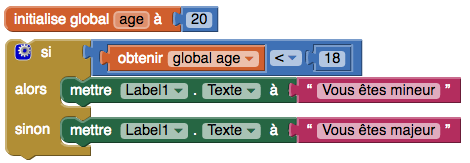
\includegraphics[scale=0.7]{if_else_exemple}
\caption{Notre exemple}
\label{exemple-if-else}
\end{figure}

Les blocs en vert foncé proviennent d'un \textbf{label} qu'il faut créer dans le \textbf{Designer}, ceux en rose de l'onglet \textbf{Texte}, les bleus de l'onglet \textbf{Math} et enfin les oranges de l'onglet \textbf{Variables}. On a ici utilisé une variable globale \texttt{age}, à laquelle on peut donner n'importe quel nombre pour définir l'âge de l'utilisateur. On vérifie ensuite sa valeur dans la condition du \texttt{si}, pour finalement afficher un des deux messages.\\

Ici, puisque l'on a mis la variable \texttt{age} à la valeur 20, la condition \textbf{ne} sera \textbf{pas} vérifiée, et c'est donc les instructions après le \texttt{sinon} qui seront exécutées. Il sera alors affiché "Vous êtes majeur" sur le \texttt{label1}. \\

\textbf{Note}~ Afin de tester ce petit exemple, il faut insérer le bloc \textit{si-sinon} quelque part. Nous suggérons de créer un bouton dans le \textbf{Designer}, puis d'insérer notre bloc \textit{si-sinon} dans l'instruction "Quand Button1.Clic ...". On peut trouver cette instruction lorsque l'on clique sous l'onglet Button1 à gauche, dans les \textbf{Blocs}. \\

Pour terminer cette partie, notons qu'il est possible de vérifier autant de conditions que l'on veut dans une structure conditionnelle. On utilise pour cela le même bloc \textit{si-sinon} que celui décrit ci-dessus, auquel on ajoute un ou plusieurs \texttt{sinon si}. On associe à \texttt{sinon si} une condition, tout comme pour un \texttt{si} ! Voyons tout de suite une application concrète : reprenons l'exemple présenté ci-dessus. On veut afficher "Vous êtes mineur" si l'utilisateur a moins de 18 ans ou bien "Vous êtes majeur" si l'utilisateur a strictement plus de 18 ans ou bien "Tout juste majeur !" si l'utilisateur a exactement 18 ans. La solution est donnée ci-dessous. Tout comme pour l'ajout du \texttt{sinon}, il suffit de cliquer sur le petit bouton bleu juste à gauche du \texttt{si} pour ajouter un \texttt{sinon si}.

\begin{figure}[h!]
\centering
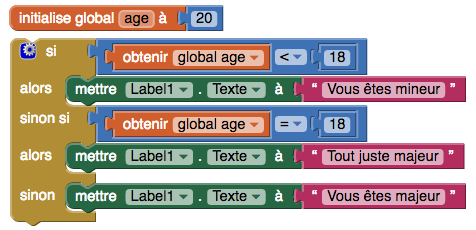
\includegraphics[scale=0.6]{exemple-elseif}
\caption{Notre exemple amélioré}
\label{exemple-elseif}
\end{figure}


\subsection{Les procédures}

Pour développer votre application, les procédures ne sont pas indispensables mais elles permettent de clarifier et simplifier ce que vous faites. Une procédure est juste une série d'instructions (des blocs). En voici un exemple~:

\begin{figure}[h!]
\centering
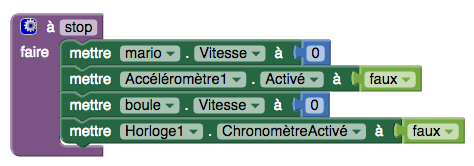
\includegraphics[scale=0.6]{exemple-proc}
\end{figure}

Cette procédure s'appelle \texttt{stop} et contient 4 instructions (blocs). Ces 4 instructions sont effectuées chaque fois qu'on \textbf{appelle} la procédure \texttt{stop}. Dans ce cas-ci, elle permet de figer certains éléments~: l'accéléromètre, la vitesse de Mario, ... Par exemple, on pourrait appeler la procédure \texttt{stop} lorsque le jeu est perdu ou gagné. Voici un exemple d'appel~:

\begin{figure}[h!]
\centering
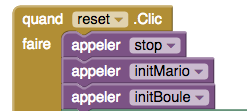
\includegraphics[scale=0.6]{exemple-proc-call}
\end{figure}

Ici, lorsque le bouton Reset est cliqué, on appelle la procédure \texttt{stop}, ce qui veut dire qu'on exécute les 4 instructions qui se trouvent dans \texttt{stop}, c'est-à-dire de mettre la vitesse de Mario à 0, d'arrêter l'accéléromètre, ... \\

Maintenant que l'on sait créer une procédure et l'appeler, nous pouvons rendre notre application plus claire et plus simple. Par exemple si vous avez une série de blocs qui se trouve à plusieurs endroits de votre application, vous pouvez~:

\begin{itemize}
\item Créer une nouvelle procédure
\item Lui donner un nom
\item Y placer la série de blocs
\item Retirer la série de blocs qui se trouve à plusieurs endroits dans votre application
\item Aux endroits où vous avez enlevé la série de blocs, y placer un \textbf{appel} à votre nouvelle procédure
\end{itemize}

\subsubsection{Les procédures avec entrée(s)}

Les procédures ont plus d'un tour dans leur sac, nous pouvons aussi leur donner une ou plusieurs \textbf{entrée(s)}. Ces entrées peuvent être utilisées par la procédure pour afficher, calculer, ... quelque chose. Voici tout de suite un exemple~:

\begin{figure}[h!]
\centering
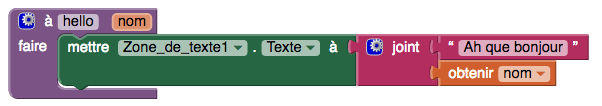
\includegraphics[scale=0.6]{exemple-proc-entry}
\end{figure}

On a définit la procédure \texttt{hello} qui prend une \textbf{entrée} qu'on appelle ici \texttt{nom}. Quand la procédure est appelée, elle change le contenu d'une zone de texte~: elle y met \textit{Bonjour} ainsi que le \texttt{nom} donné en entrée. En voici un exemple d'utilisation~:

\begin{figure}[h!]
\centering
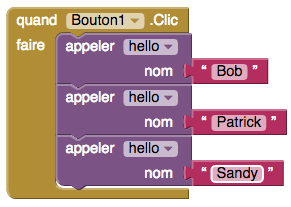
\includegraphics[scale=0.6]{exemple-proc-entry-call}
\end{figure}

Ici on appelle 3 fois la procédure \texttt{hello}. Après le premier appel, le contenu de la zone de texte sera \textit{Bonjour Bob}, après le deuxième appel, le contenu sera \textit{Bonjour Patrick} et enfin après le troisème appel, le contenu sera \textit{Bonjour Sandy}.

\clearpage
\subsection{Les boucles}
Les boucles sont très utilisées en informatique pour répéter une opération. On va répéter cette opération tant qu'une condition n'est pas vérifiée. Par exemple, lorsque l'on doit faire une punition qui consiste à écrire 500 fois "Je ne parlerai pas en cours", il suffit d'utiliser une boucle qui écrit "Je ne parlerai pas en cours" tant que cela n'a pas été fait 500 fois, et qui s'interrompt ensuite.\\

Les 2 boucles les plus utilisées en informatique sont les boucles \texttt{tant que} et \texttt{pour}. Les boucles \texttt{pour} sont en fait un type particulier de boucles \texttt{tant que}.\\

La boucle \texttt{tant que} effectue une opération tant qu'une condition n'est pas respectée. Par exemple, si l'on veut jouer un son tant que l'utilisateur n'a pas appuyé sur un bouton, on écrira quelque chose comme~:

\begin{center}
\texttt{tant que} "l'utilisateur n'a pas appuyé sur le bouton", \texttt{faire} "jouer le son".
\end{center}

Tant que l'utilisateur n'appuie pas, le son sera joué encore et encore, et une fois que l'utilisateur aura appuyé sur le bouton, on sortira de la boucle et le son arrêtera d'être joué. \\

La boucle \texttt{pour} est presque identique à la boucle \texttt{tant que}, sauf qu'elle inclut un compteur. En voici un exemple~: 

\begin{figure}[h!]
\centering
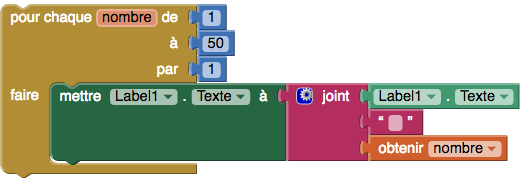
\includegraphics[scale=0.7]{forloop.png}
\end{figure}

Dans cet exemple, une variable appelée \texttt{nombre} dont la valeur initiale est 1, sera incrémentée de 1 (+1) à la fin de chaque exécution du contenu de la boucle (dans le \texttt{faire}), jusqu'à ce qu'elle vaille 50. La condition à respecter pour rester dans la boucle est que \texttt{nombre} soit compris entre 1 et 50.
Lorsque l'on rentre dans la boucle, on aura donc \texttt{nombre} initialisé à 1, puis 1 qui sera écrit dans le \textit{label1}. Ensuite, \texttt{nombre} sera incrémenté de 1, on aura donc \texttt{nombre}=2. La condition étant toujours vérifiée (\texttt{nombre} est compris entre 1 et 50), on repassera dans le \texttt{faire}, et on va donc afficher 2 à côté de 1 dans le \textit{label1}. Puis à nouveau, \texttt{nombre} sera incrémenté. Au final, on obtiendra donc une suite des nombres de 1 à 50 dans notre \textit{label1}. Une fois que \texttt{nombre} vaudra 51, la condition ne sera plus respectée, et on va donc sortir de la boucle, sans exécuter l'opération.

\subsection{Divers}
Cette dernière partie mentionne quelques éléments intéressants à utiliser sur App Inventor 2. N'hésitez pas à les tester par vous-mêmes !
\subsubsection{Horloge}
L'utilisation d'une \texttt{horloge} permet d'effectuer une action à intervalles réguliers. On peut la voir comme une boucle qui s'active à intervalles réguliers. Une \texttt{horloge} peut être démarrée ou arrêtée et on peut changer sa fréquence. On utilise un bloc \texttt{Quand Horloge.Chronomètre faire} pour définir ce que l'on veut qu'il se passe toutes les 2 secondes par exemple. On peut bien sûr choisir si cela doit arriver toutes les 1, 2, 10 secondes, à volonté. On utilise pour cela l'\texttt{IntervalleChronomètre}, disponible dans l'onglet \textbf{Designer}. On peut aussi le changer au cours de l'utilisation de l'application.

\subsubsection{Cadre}
Un \texttt{cadre} est une zone de travail. Dans cette zone on peut mettre des \texttt{balles} et des \texttt{Images lutins}. Les premières sont simplement des balles, et les suivantes sont des images que l'on peut \textit{charger} depuis son ordinateur. Ces deux éléments sont présentés après cette section. Un \texttt{cadre} permet de faire plusieurs choses~: on y place des éléments qui peuvent bouger, on détecte des mouvements de doigts, des touches à l'écran,... \\

Il est aussi à noter que le système d'axe (X,Y) est un peu particulier. L'origine (0,0) se trouve tout en haut à gauche du \texttt{cadre} dans lequel les éléments évoluent. De plus, les Y augmentent en \textbf{descendant}. Ce qui veut dire que si votre écran fait 200 pixels de longueur et 100 pixels de largeur, le point tout en \textit{bas à droite} possède les coordonnées (100,200). Ce système de coordonnées est valable pour n'importe quel objet dans votre application !

\subsubsection{Balle}
Une \texttt{balle} est simplement une balle qui peut bouger dans un \texttt{cadre}. On peut lui attribuer une vitesse et une orientation, lui permettre de bouger ou la stopper (\texttt{Activée}), mais également définir ce qu'elle doit faire lorsqu'on la touche ou qu'on la déplace. Il est aussi possible de définir ce qu'elle doit faire lorsqu'elle touche un bord de l'écran~: la faire rebondir par exemple. Il est important de noter que les bords de l'écran possèdent un numéro particulier et que la direction se donne en \textbf{degrés}. Voici une image qui nous donne les informations nécessaires~:

\begin{figure}[h!]
\centering
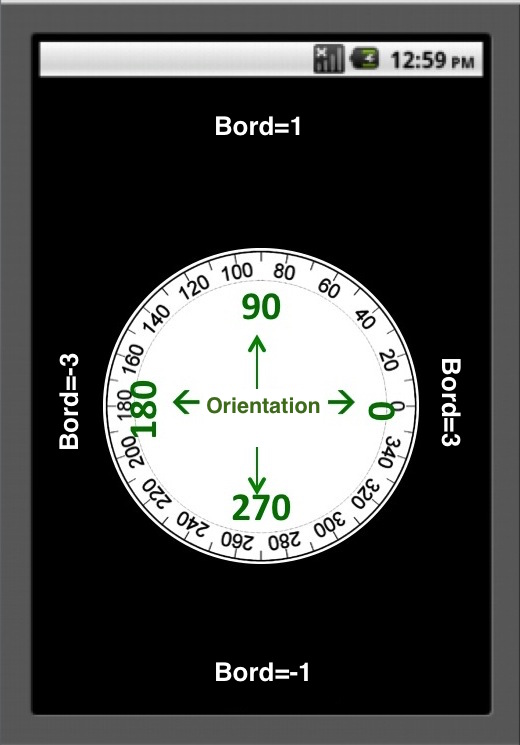
\includegraphics[scale=0.3]{edges_headings_diagram.jpg}
\end{figure}

\subsubsection{Image lutin}
Une \texttt{Image lutin} n'est rien de plus qu'une image que vous fournissez depuis votre ordinateur. On peut définir ce qu'il se passe lorsqu'on la touche ou qu'on la déplace. \\

Vous en savez désormais assez pour vous lancer dans une application Android avec App Inventor 2, c'est en testant vous-mêmes tout ce qui a été présenté (et bien plus encore) que vous apprendrez le mieux. C'est parti !

\end{document}
